\documentclass[]{article}
\usepackage{lmodern}
\usepackage{amssymb,amsmath}
\usepackage{ifxetex,ifluatex}
\usepackage{fixltx2e} % provides \textsubscript
\ifnum 0\ifxetex 1\fi\ifluatex 1\fi=0 % if pdftex
  \usepackage[T1]{fontenc}
  \usepackage[utf8]{inputenc}
\else % if luatex or xelatex
  \ifxetex
    \usepackage{mathspec}
  \else
    \usepackage{fontspec}
  \fi
  \defaultfontfeatures{Ligatures=TeX,Scale=MatchLowercase}
\fi
% use upquote if available, for straight quotes in verbatim environments
\IfFileExists{upquote.sty}{\usepackage{upquote}}{}
% use microtype if available
\IfFileExists{microtype.sty}{%
\usepackage{microtype}
\UseMicrotypeSet[protrusion]{basicmath} % disable protrusion for tt fonts
}{}
\usepackage[margin=1in]{geometry}
\usepackage{hyperref}
\hypersetup{unicode=true,
            pdftitle={Prevention through Design (PtD) to Make Solar-Ready Houses Safe for Solar Workers},
            pdfauthor={Hyun Woo Lee, John Gambatese, Yohan Min},
            pdfborder={0 0 0},
            breaklinks=true}
\urlstyle{same}  % don't use monospace font for urls
\usepackage{graphicx,grffile}
\makeatletter
\def\maxwidth{\ifdim\Gin@nat@width>\linewidth\linewidth\else\Gin@nat@width\fi}
\def\maxheight{\ifdim\Gin@nat@height>\textheight\textheight\else\Gin@nat@height\fi}
\makeatother
% Scale images if necessary, so that they will not overflow the page
% margins by default, and it is still possible to overwrite the defaults
% using explicit options in \includegraphics[width, height, ...]{}
\setkeys{Gin}{width=\maxwidth,height=\maxheight,keepaspectratio}
\IfFileExists{parskip.sty}{%
\usepackage{parskip}
}{% else
\setlength{\parindent}{0pt}
\setlength{\parskip}{6pt plus 2pt minus 1pt}
}
\setlength{\emergencystretch}{3em}  % prevent overfull lines
\providecommand{\tightlist}{%
  \setlength{\itemsep}{0pt}\setlength{\parskip}{0pt}}
\setcounter{secnumdepth}{0}
% Redefines (sub)paragraphs to behave more like sections
\ifx\paragraph\undefined\else
\let\oldparagraph\paragraph
\renewcommand{\paragraph}[1]{\oldparagraph{#1}\mbox{}}
\fi
\ifx\subparagraph\undefined\else
\let\oldsubparagraph\subparagraph
\renewcommand{\subparagraph}[1]{\oldsubparagraph{#1}\mbox{}}
\fi

%%% Use protect on footnotes to avoid problems with footnotes in titles
\let\rmarkdownfootnote\footnote%
\def\footnote{\protect\rmarkdownfootnote}

%%% Change title format to be more compact
\usepackage{titling}

% Create subtitle command for use in maketitle
\newcommand{\subtitle}[1]{
  \posttitle{
    \begin{center}\large#1\end{center}
    }
}

\setlength{\droptitle}{-2em}

  \title{Prevention through Design (PtD) to Make Solar-Ready Houses Safe for
Solar Workers}
    \pretitle{\vspace{\droptitle}\centering\huge}
  \posttitle{\par}
    \author{Hyun Woo Lee, John Gambatese, Yohan Min}
    \preauthor{\centering\large\emph}
  \postauthor{\par}
      \predate{\centering\large\emph}
  \postdate{\par}
    \date{May 25, 2019}

\usepackage{booktabs}
\usepackage{longtable}
\usepackage{array}
\usepackage{multirow}
\usepackage{wrapfig}
\usepackage{float}
\usepackage{colortbl}
\usepackage{pdflscape}
\usepackage{tabu}
\usepackage{threeparttable}
\usepackage{threeparttablex}
\usepackage[normalem]{ulem}
\usepackage{makecell}
\usepackage{xcolor}

\usepackage{float}
\floatplacement{figure}{H}
\usepackage[fontsize=11pt]{scrextend}

\begin{document}
\maketitle

\hypertarget{introduction}{%
\section{Introduction}\label{introduction}}

Solar installation in the U.S. has increased dramatically in recent
years. Specific to the residential sector, the number of houses with
solar modules increased exponentially from 30,000 homes to 1 million
homes in 10 years from 2006 to 2016, with record growth in 2015
(Harrington 2015; GTM/SEIA 2017). Most solar installations in the
residential sector happen on small, sloped roofs and as a result,
installers are subject to unique safety concerns in terms of existing
roof conditions. Furthermore, the installation process involves roofing,
electrical and mechanical work, and IT causing hazards to installers. To
prevent those unique safety hazards and risks, especially related to
fall hazards during solar installations, a previous The Center for
Construction Research and Training (CPWR)-supported small study
conducted by the researchers investigated how Prevention through Design
(PtD) can be applied to solar design and installation for small
buildings (Lee et al.~2017). The small study led to the identification
of seven PtD attributes based on roof conditions and rooftop solar
system (hereafter solar system) characteristics: roofing material, roof
slope, roof accessory, module layout, fall protection system, lifting
method, and electrical system. Based on the identified PtD attributes,
the researchers developed a PtD protocol for solar installer safety. For
broader nationwide dissemination, the protocol was presented through a
CPWR webinar on December 13, 2017.

While the previous study focused on applying PtD to existing houses, the
study actually revealed that to maximize the efficacy of PtD for solar
installer safety, the application of PtD should also be considered for
new houses as a way to make them solar-ready. To that end, during the
final seminar conducted in the small study, the research team asked
solar contractors what house features would make residential solar
installation safer. The followings are excerpts from some of their
responses:

\begin{itemize}
\tightlist
\item
  ``Nothing extruding from the roof on the south side of the house''
\item
  ``No shake roofs, no tile roofs''
\item
  ``Having roof anchors or anchor points ready''
\item
  ``Pre-wired for solar system electrical connections''
\end{itemize}

Making new commercial buildings solar-ready has become a requirement in
cities like Seattle, WA, and San Francisco, CA. These cities are
mendating solar-ready to the residential sector as well. Phoenix
Building Construction Code added solar-ready provisions to detached one
and two family dwellings on proposed amendment to the 2018 Internatial
Residential Code (IRC). Furthermore, California's 2019 residential
building energy efficiency standards include solar installation mendate
and solar-ready for all residential buildings. Currently, there are some
guidelines available to support the design of solar-ready buildings
(e.g., Watson et al.~2012, EPA 2011; Lisell et al.~2009). However, the
current literature largely lacks considerations of the safety of solar
installers, and hence the application of PtD to solar-ready houses has
been significantly limited. In response, this study aims to fill this
knowledge gap by developing a design checklist to apply PtD to the
design of houses to make them both solar-ready and safer for solar
installations. The results of the previous CPWR study (Lee et al.~2017)
significantly contributed to the successful completion of the study by
serving as a foundation for the development of the design checklist. In
particular, the study is expected to showcase how the design community
can be involved in promoting the concept of PtD during the design of
green buildings that pursue sustainability and energy efficiency.

\hypertarget{research-objectives}{%
\section{Research objectives}\label{research-objectives}}

The overall objective of the study is to develop knowledge and resources
that support the application of PtD to the design of new solar-ready
houses. The study is expected to provide evidence that (1) PtD can
improve solar installer safety by proactively eliminating safety hazards
and mitigating risk; and (2) designers can proactively get involved in
promoting PtD for solar-ready houses.

Using mixed methods, the specific tasks of the research are as follows:

\begin{enumerate}
\def\labelenumi{\arabic{enumi}.}
\tightlist
\item
  Perform literature review
\item
  Investigate design features for solar safety
\item
  Categorize the components of solar-ready houses
\item
  Perform case studies of existing solar-ready houses
\item
  Develop a PtD design checklist and BIM (building information model)
  for new solar-ready houses
\item
  Obtain industry feedback on the checklist and model
\item
  Develop and submit a final report
\end{enumerate}

\hypertarget{perform-literature-review}{%
\section{Perform literature review}\label{perform-literature-review}}

An extensive literature review was conducted to identify (1) the design
components and construction operations of solar-ready houses, and (2)
the safety hazards and risk mitigation measures for solar systems. Seven
PtD components identified in the previous study (Lee et al.~2017) are:
roofing material, roof slope, roof accessories, module layout, fall
protection system, lifting method, and electric system. These components
were identified with respect to the three main safety hazards, which are
falling, tripping, and being struck by objects. The hazards are
prevalent specifically when working on a rooftop due to a variety of
factors including, but not limited to, stability of the roof, placement
of the ladder, weather conditions, openings in the roof, proximity of
the roof edges, and pitch of the roof. These factors were considered for
the next steps in the development of desirable design features and a
design checklist of solar-ready houses.

In addition, energy codes were reviewed to identify the safety features
in the requirements. Each state has adopted or developed energy code
from the federal government's energy standard such as International
Energy Conservation Code (IECC). California has its own standards, the
2016 Building Energy Efficiency Standards Title 24, Part 6, which
exceeds the requirements of 2015 IECC. California requires rooftop solar
installation on new construction or solar-ready for those who are exempt
from the solar installation (CEC 2016). The newly updated 2018 IECC has
APPENDIX RA solar-ready provisions, which include solar ready
requirements for detached, and one and two family dwellings and
townhouses (IECC 2018). The 2017 residential code is in effect in
Seattle (Seattle 2017). The requirements for residential solar-ready are
in residential code while commercial solar-ready requirements are in
energy code, not building code. For reference, single family and low
rise multifamily are related to residential code (a kind of building
code only for residential) otherwise building code. Electrical permit,
which is related to electrical code from National Electric Code (NEC),
is required when a solar system is installed.

Solar-ready requirements, in general, found in these energy codes mainly
focus on securing solar zones for the easier implementation and
installation in the future considering dimension, area and orientation.
A solar zone refers to a designated area for the future installation of
solar modules on the roof or overhang without interruption due to shade,
penetrations, and obstructions (CEC 2016). These codes demand solar zone
to be larger than a certain area depending on the total available roof
area in addition to load, electric interconnection, and documentation
requirements. While these requirements are primarily to ensure reserved
spaces for the future solar modules on the roof, having solar zones
itself is expected to entail occupationally safer conditions for
installers to install the system. It is because securing a solar zone
will prevent any obstructions from occurring on the roof where a solar
system is going to be installed. Obstruction on roof is the one of
factors causing tripping hazards.

\hypertarget{investigate-design-features-for-solar-safety}{%
\section{Investigate design features for solar
safety}\label{investigate-design-features-for-solar-safety}}

A series of interviews with industry practitioners were performed to
capture specific features that can be considered for improved safety of
solar installations. All located in the Pacific Northwest, the
interviewees were identified through the previous CPWR study and the
research team's connections with industry. The team tried to select a
diverse set of the professionals for interviews so as to capture broad
perspectives from the field installers to the company principals. A
total of 12 industry professionals were interviewed. The interviewees
included one sustainability consultant, three solar contractors, one
general contractor, two electric professionals, and five designers
(including two principals).

\begin{table}[t]

\caption{\label{tab:unnamed-chunk-1}List of interviews}
\centering
\begin{tabular}{r|l|>{\raggedleft\arraybackslash}p{1em}|l|l|>{\raggedleft\arraybackslash}p{1em}}
\hline
No. & Position & No. of contacts & Date & Location & Duration (hour)\\
\hline
1 & Electrical & 1 & 2018-10-15 & Coffee shop, Seattle & 1.0\\
\hline
2 & Designer & 3 & 2018-10-20 & Via phone call, Hawaii & 1.0\\
\hline
3 & Designer & 1 & 2018-10-22 & Coffee shop, Seattle & 1.0\\
\hline
4 & Consultant & 1 & 2018-10-22 & UW campus, Seattle & 1.5\\
\hline
5 & Electrical & 2 & 2018-10-25 & Site office, Renton & 1.0\\
\hline
6 & Solar contractor & 3 & 2018-10-26 & Site office, Seattle & 2.0\\
\hline
7 & Solar contractor & 2 & 2018-10-30 & Site office, Seattle & 1.0\\
\hline
8 & Solar contractor & 2 & 2018-11-04 & Coffee shopt, Seattle & 1.5\\
\hline
9 & Designer & 1 & 2018-11-06 & Site office, Seattle & 1.0\\
\hline
10 & General contractor & 1 & 2018-11-30 & Site office, Seattle & 1.0\\
\hline
11 & Designer & 1 & 2018-12-03 & UW campus, Seattle & 1.0\\
\hline
12 & Designer & 2 & 2018-12-12 & Site office, Seattle & 1.0\\
\hline
\end{tabular}
\end{table}

The interviews led to identification of design features with
recommendations to improve safety of installers for rooftop solar
installation.

\hypertarget{roof-area}{%
\subsection{Roof area}\label{roof-area}}

First, it is confirmed that there should be no obstruction around roof
area where a solar system is going to sit on to avoid a trip hazard.
Mounting accessories such as foots for racks and rails, could be
pre-installed. Having simple roof shape is preferred for the sake of
solar installers. For a complicated roof shape, the use of composition
material would make the installation work easier and safer. It would be
safer to have access gaps between modules for installers to walk around
during the work.

\hypertarget{roof-pitch-and-flat-roof}{%
\subsection{Roof pitch and flat roof}\label{roof-pitch-and-flat-roof}}

When it comes to roof pitch, lower than 5/12 -- 7/12 (depending on the
roofing material and climate) was suggested for the safety of solar
installers while the optimal pitch for energy production is depending on
the local attitude (8/12 is the optimal in Northwest). If it is a lower
pitch, any roofing material would be fine in terms of safety. There
were, however, some concerns about flat roof because they may require
the use of ballast mounting for solar modules. Additional structural
analysis would be required for flat roof in order to accommodate ballast
mounting structures and their weights. In addition, if solar
installation on flat roof requires membrane penetration, water intrusion
issues should be verified by a roofing expert. A solar system with
ballast mounting may also incur additional engineering cost and a
building permit. Furthermore, flat roof is a bit harder to have overhang
while overhang is necessary in a climate such as Seattle to protect a
house from the frequent rain while. It was told that accessing flat roof
would be harder because most residential houses with flat roof are, in
general, taller in order for securing more space on the top floor level.

\hypertarget{roof-material}{%
\subsection{Roof material}\label{roof-material}}

Composition, overall, is better for safety since it is easier to work
on, leading to less slippery condition while composition was told poor
in maintenance. It is because composition involves moss growth, and it
is less durable, which incurs replacement of the roofing material and
reinstallation of solar modules costing 25\% of the initial cost for
labor. Durable roofing material is suggested to be metal although it
could be slippery to walk on and may cause heatstroke during Summer. In
general, typical metal roof entails no penetration to install a solar
system that makes solar installers easier and safer to work. On the
other hand, tile and shake are easy to crack and it takes longer to
install a solar system on them. In addition, shakes have a fire hazard.
Housing aesthetics is, with the development of modern design, the other
factor to consider for the roofing material.

\hypertarget{fall-protection-and-access}{%
\subsection{Fall protection and
access}\label{fall-protection-and-access}}

Anchor points or tie-offs are suggested to be pre-installed on rooftop
as it would be more dangerous to install them after construction. There
is, however, a liability issue for homeowners to install the anchor
points such that any accidents related to the homeowner-installed
tie-offs could endanger the homeowner in regard to reliability and
maintenance of the tie-offs, which are not required to be installed in
building code. There were additional options recommended such as access
pathway, snow guard and guardrail as the means of fall protection.
Access pathways are required by International Fire Code (IFC)
605.11.3.2, if certain conditions were not met. For the purpose of
safety, it is better to have access pathways for accessing and securing
space on roof even if access pathways are not required to have. Lower
height was told to be better for safety. Creative access point may be
needed depending on the house neighbors for delivery of material and
people because some house neighbors are close each other having no space
to put a ladder. Lower pitch makes easier access in this regard by
allowing a gentle slope of a ladder.

\hypertarget{electrical-issues}{%
\subsection{Electrical issues}\label{electrical-issues}}

Overhead powerlines is another factor to watch out during the work. A
recent incident cited by Occupational Safety and Health Administration
(OSHA) about fatal electrocution, leads to the company facing penalties
at Kansas (EC\&M 2019). ``This tragedy could have been prevented if the
employer had complied with electrical standards that require maintaining
a safe distance from unprotected energized power lines, training
employees, and providing personal protective equipment,'' said OSHA
Wichita Area Director Ryan Hodge. Conduit for a solar system is
suggested to be pre-run because it would be easier to run them during
new construction with less manpower. It will be complicated to run
conduit internally by opening walls in the future. Aesthetics is the
other factor to consider for conduit and inverter location. Reserving
spaces for electric equipment on the same side or near was recommended.
In regard to inverter type, the concern was more about economical
efficiency such that micro inverter and power optimizer are preferred
for small system such as less than 35 solar modules, otherwise string
inverter is suggested for systems like commercial projects. Micro
inverter and power optimizer are also safer in terms of rapid shutdown,
which is required to disperse direct current (DC) for a short period of
time (all conductors within an array's 1-ft boundary have to be reduced
to 80 V or less within 30 seconds of rapid shutdown initiation - NEC
2017).

In summary, the interview results revealed that most safety hazards and
risks happen during the installation of the safety equipment such as
tie-off and anchor points and during the process of carrying solar
modules to the roof. Typical solar system installation starts with
installing safety equipment followed by installation of mechanical and
electrical balance of system (BOS) such as mounting racks and an
overcurrent protection device (OCPD). Carrying and positioning solar
modules are the next step followed by installation of final accessories.
Hence, the application of PtD to the design features would help to
address these hazardous activities effectively during the design
process.

\hypertarget{categorize-the-components-of-solar-ready-houses}{%
\section{Categorize the components of solar-ready
houses}\label{categorize-the-components-of-solar-ready-houses}}

A list of building components pertaining to the identified design
features were first identified through the interviews. Then, an online
survey was performed to rank the design features preferred by industry
practitioners including those who participated in the previous
interviews. The ranking was based on evaluation criteria including (1)
relevance to safety hazard risks, (2) applicability, and (3)
cost-effectiveness. The relevance to safety hazard risks is a criterion
to measure how safe it is to have the concerned component for installer
safety. Applicability is a criterion that leads to the easiest
application in practical. Cost-effectiveness refers to the most
economical option. Based on the interviews, the identified design
features are grouped into eight categories (solar zone area, solar zone
material, solar zone pitch, fall protection, access to roof, conduit for
the future rooftop solar, solar system inverter, and solar system
mounting) to specify which feature in each section is the most
desirable.

\hypertarget{solar-zone-area}{%
\subsection{Solar zone area}\label{solar-zone-area}}

Safety hazards are trip, fall, and complexity. The majority of
professionals consider one continuous zone is more desirable than the
multi-split zones for all criteria. One of the reasons was captured that
given the same size of system, installation of the system in several
areas would complicate the work and incur installation of additional
accessories.

\hypertarget{solar-zone-material}{%
\subsection{Solar zone material}\label{solar-zone-material}}

Safety hazards are slip, fire, heat stroke, complexity, rework, and
maintenance. Composition is the most desirable in the safety criteria
while metal (standing seam) is the one as far as applicability is
concerned. When it comes to the cost-effectiveness, composition and
metal are considered almost the same. In general, metal is expensive
with higher upfront cost. Metal, however, could be cost-effective as
much as composition with respect to durability and maintenance in a long
run.

\hypertarget{solar-zone-pitch}{%
\subsection{Solar zone pitch}\label{solar-zone-pitch}}

Safety hazards are slip, fall, complexity, and maintenance. Flat is the
safest feature for solar zone pitch in the survey. Lower slope is
desirable in cost-effectiveness criteria. OSHA defines a low-slope roof
as a roof having a slope of less than or equal to 4 inches of vertical
rise for every 12 inches horizontal length (standard no. 1926.500).

\hypertarget{fall-protection}{%
\subsection{Fall protection}\label{fall-protection}}

Safety hazards are slip and fall. Hitch clip or tie-off (anchor point)
is the feature chosen the most for all the criteria of safety,
applicability and cost-effectiveness. There were other suggestions such
as guardrail and snow guard for the safety criteria. Snow guard could be
the mean of footholds for installers to step on while it is originally
to allow snow and ice to drop off or melt in small amounts before
falling to the ground. The installation of snow guards prevents the
sudden release of snow and ice from a roof.

\hypertarget{access-to-roof}{%
\subsection{Access to roof}\label{access-to-roof}}

Safety hazards are slip, trip, and fall. Ladder is the most desirable
for the cost-effectiveness and applicability criteria while none
selected ladder when safety is concerned, but other options such as
scaffolding and mechanical lift. There are trade-offs between safety and
economical efficiency or applicability.

\hypertarget{conduit-for-the-future-solar-system}{%
\subsection{Conduit for the future solar
system}\label{conduit-for-the-future-solar-system}}

Safety hazards are complexity and rework. Most of respondents vote for
running conduits in advance for safety, applicability and
cost-effectiveness. This goes along with one of the suggestions during
the interview process that internal installation of conduit after
construction would cause more cost and labor work while outdoor
installation may harm the housing aesthetics.

\hypertarget{solar-system-inverter}{%
\subsection{Solar system inverter}\label{solar-system-inverter}}

Safety hazards are fall, trip, and electrocution. Micro inverter was
chosen as the most desirable in the safety criteria. When it comes to
applicability and cost-effectiveness, there are not much differences
among the features. In practice, the desirable inverter would be
different depending on the solar system size and the roof condition.
Larger capacity of the system such as commercial projects, would need
string inverters. Micro inverter and power optimizer are more desirable
for smaller systems and in the more dynamic conditions such as
situations with marginal shading and complicated roof. Micro inverter
leads to having many electronic components on roof ending up with more
maintenance cost. Power optimizer, on the other hand, accompanies a
central inverter while having the similar performance to the micro
inverter. The point is where the inverter converts DC to alternating
current (AC). Micro inverter does it on roof which leads to the safest
feature among the other inverter options on the electrical safety
perspective. Micro inverter or power optimizer, however, can pose a trip
hazard as they accompany more electronic components up on the roof
unlike the string inverter option. A string inverter requires installers
stay comparatively less time on roof, thus could reduce potential risks
present on the roof.

\hypertarget{solar-system-mounting}{%
\subsection{Solar system mounting}\label{solar-system-mounting}}

Safety hazard is heavy lifting. Racking type is more desirable than
ballast type for applicability and cost-effectiveness. There was not
difference between the options for the safety criteria. There were some
opinions that the ballast mounting may lead to carrying heavy objects on
a ladder to roof, which may incur a dangerous situation.

\begin{figure}
\centering
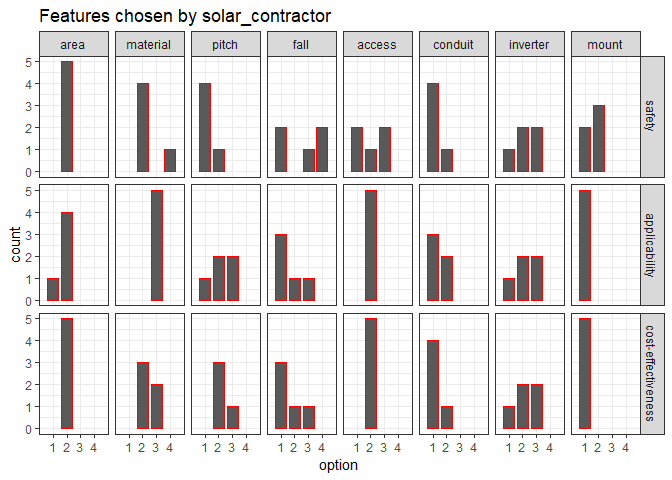
\includegraphics{reportA_files/figure-latex/unnamed-chunk-2-1.pdf}
\caption{Survey results (area: 1 is multi-split zones and 2 is one
continuous zone; material: 1 is tile or shake, 2 is composition, 3 is
metal, and 4 is others; pitch: 1 is flat, 2 is lower (less than 4/12), 3
is moderate (between 4/12 to 8/12), and 4 is steep (more than 8/12);
fall: 1 is hitch clip or tie-off, 2 is roof bracket, 3 is lifeline, and
4 is others; access: 1 is scaffolding, 2 is ladder, and 3 is mechanical
lift; conduit: 1 is running in advance and 2 is routes decided but not
running; inverter: 1 is string inverter, 2 is power optimizer, and 3 is
micro inverter; mount: 1 is rack and 2 is ballast)}
\end{figure}

The survey aimed to evaluate the desirable design features in each of
the eight building components. General contractors, who mainly work on
commercial projects, seem to prefer flat and ballast to other options
regardless of criteria. Other material options and ballast mounting
types are likely determined by the design of roof pitch such that flat
pitch would entail TPO (Thermoplastic polyolefin, a single-ply roofing
membrane covering the surface of the roof) or other similar materials
(EPDM and PVC) as well as ballast mounting for a solar system. It is
because composition or metal are hardly used for flat roof in
consideration of additional water proof medium necessary to the flat.

There are conflicts among the most desirable features in the different
building components and objectives in regard to safety. Features such as
composition material, flat pitch, scaffolding or mechanical lift to
access roof, and micro inverter are the most desirable in an independent
perspective for safety. The most desirable combined set of features,
however, could be various and context-dependent. For example,
composition material is considered to be safer but it results in
penetration on roof adding additional mounting foots while metal
material isn't mainly involved with the penetration. Scaffolding and
mechanical lift are safer, but they are generally not applicable in
consideration of economic efficiency. Overall, continuous solar zone,
tie-off for fall protection, and running conduit in advance are the
features to enhance the safety in current practice.

\hypertarget{perform-case-studies-of-existing-solar-ready-houses}{%
\section{Perform case studies of existing solar-ready
houses}\label{perform-case-studies-of-existing-solar-ready-houses}}

Case studies were performed to verify the findings through the previous
interviews and survey to the real world applications. A total of four
houses were chosen for this study. It should be noted that three out of
the four houses were acknowledged for the U.S. Department of Energy
(DOE) Housing Innovation Award in 2013, 2015, and 2016 respectively in
order of Case Study 1, 2 and 3 for their energy efficiency, production
and environmental-friendly features. Two houses are certified 5-Star
Built Green, which refers to 30\% energy use improvement above current
Washington State Code in addition to pre-wired for any future solar
installations for single-family houses. Case Study 3 is certified with
Emerald Star Built Green, which achieved net zero energy using a
renewable source in addition to 70\% reduction in water use, 90\%
reclaimed or FSC certified wood materials, and higher indoor air
quality. These three Case Studies were chosen to represent solar-ready
houses. Case Study 4 represents a typical residential single-family
house that was not built for solar-ready.

Figures below show the satellite images of google map for the solar
modules installed on the roof of these case studies. Note that the
figure of Case Study 4 does not show any solar modules installed due to
the fact that the google map was not updated since the house installed
the solar modules in 2018.

\begin{figure}
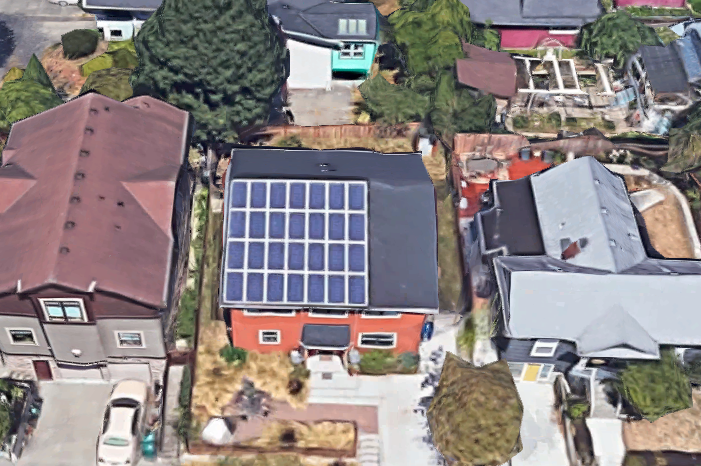
\includegraphics[width=3.12in]{../case/case1/google} 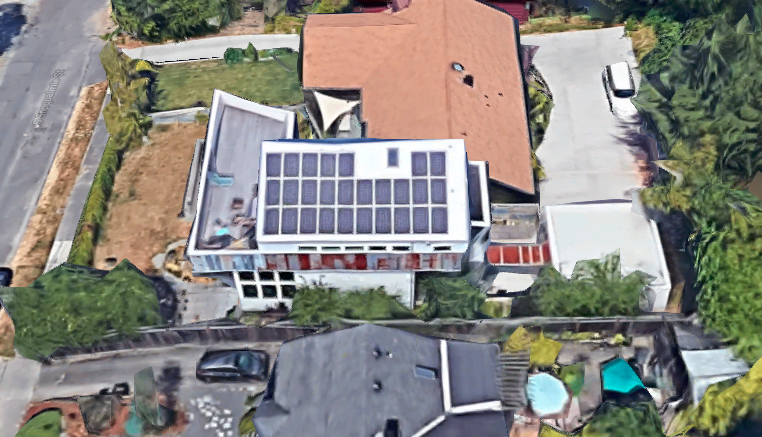
\includegraphics[width=3.63in]{../case/case2/google} \caption{Case Studies 1 and 2 (Google map accessed in 2019)}\label{fig:unnamed-chunk-3}
\end{figure}

\begin{figure}
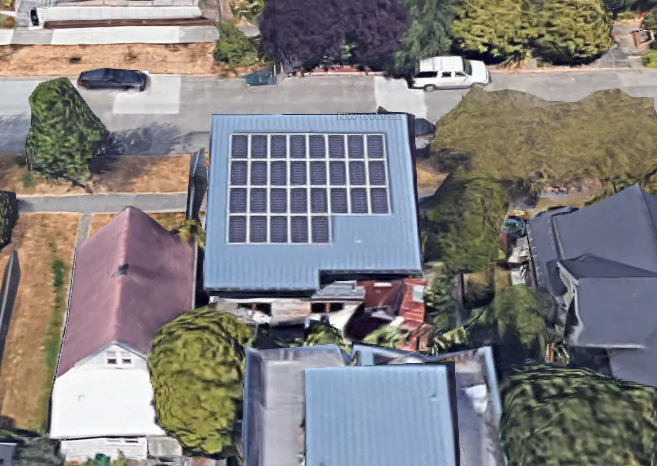
\includegraphics[width=2.95in]{../case/case3/google} 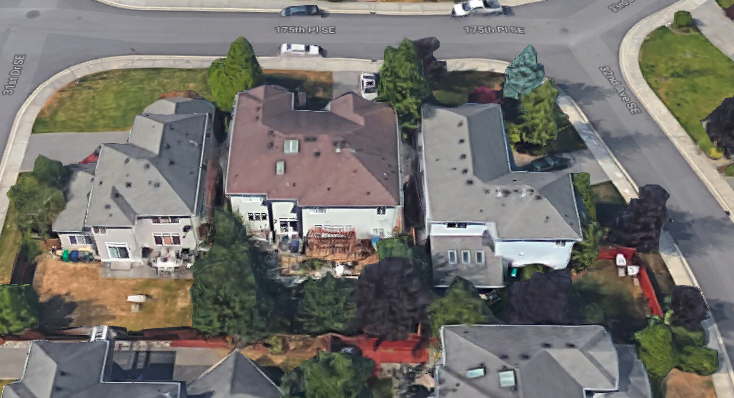
\includegraphics[width=3.86in]{../case/case4/google} \caption{Case Studies 3 and 4 (Google map accessed in 2019)}\label{fig:unnamed-chunk-4}
\end{figure}

\hypertarget{case-study-1}{%
\subsection{Case Study 1}\label{case-study-1}}

In the first case study, south facing roof where solar modules are
installed is 22' from top to bottom of the roof panel as measured along
the plane of the roof and 36' wide. The roof pitch on the side of the
roof with the solar modules is 4/12 and the back side of the roof is
7/12, which is on north side and has almost the same roof area. In the
interview it was told that there is little difference at Pacific
Northwest in terms of latitude and the climate zone in energy production
between a 4/12 pitch and an 8/12 pitch. ``It is more about convective
loop that is developed in the two-story great room providing for passive
distribution of the in-floor radiant heat to the upstairs rooms'' says
the principal who designed the house. The live load of the roof is 25
lbs for snow, 5 lbs for the solar modules, and 15 lbs for the structural
insulated panels (SIPs), total of 45 lbs. Permanent tie-offs or anchor
points were installed on the rooftop. Normal way to access the roof of
this house is by a ladder. It was told that there was no issue for the
solar contractor interacting with roofers with respect to the design and
installation of the solar system.

Automated fire sprinkler in regard to fire code to have 3 ft setbacks
from roof edges and ridges was not needed in the case study. There were
certain circumstances leading to exemption such as roofs with less than
30\% total solar module coverage, and when the fire marshal determines
that having a fire-fighter on the roof is not necessary. ``That is
always the case with a SIPs roof. Fire-fighter should never be on top of
a SIPs that is on fire, because if the bottom skin of the SIPs fails,
the entire roof fails. Because there is no enclosed roof truss space
that could house a fire, there is no need to ventilate the roof as they
would a structure with a trussed or stick-framed roof'' says the
designer.

Unlike other case studies amoung solar-ready houses (Case Study 1, 2 and
3), Case Study 1 has conduit run on outside wall with outdoor electric
equipment. The designer confirmed that the reason to install solar
electrical balance of systems (BOS) outside is that it would be easier
to add more solar modules and another inverter in the future in
consideration of charging an electric car if the BOS were outside. They
are located on the West wall. Furthermore, this case study has a string
inverter installed instead of micro inverter, which is the cases for the
other two case studies (Case Study 2 and 3). Another difference is that
it doesn't have access pathways along the lines of the roof eave and
edge. Although it doesn't violate the IFC code by having access pathways
the other sides, it is still suggested to have access pathways for safer
working condition on the roof.

\hypertarget{case-study-2-and-3}{%
\subsection{Case Study 2 and 3}\label{case-study-2-and-3}}

The other two case studies as being solar-ready houses, have access
pathways around solar zones. Their roofing materials are all metal
(standing seam) leading to no penetration of mounting foot for the solar
modules to be installed. Electrical conduit is run inside walls, thus
not visible on the walls. Their inverter systems are micro inverters
installed with solar modules on the roof where DC generated from the
modules is converted to AC. It was told that it took about 2 to 3 days
to install the solar modules and systems at the end of the construction.
The roof design and access to roof are different While they share the
similar characteristics of the housing design and the solar system due
to the fact that the designer and builder of the houses and the solar
contractors are the same for the both houses. Case Study 2 could take
advantage of the deck on the 3rd floor level to put a ladder for
accessing the roof. This could be considered in design process to allow
people easier to access the roof by providing a deck to put a ladder on.
The house, however, has a higher roof pitch, 8/12 where solar modules
sit on and has a single skylight. The shade impact from the height of
the skylight is trivial considering the shading equation of distance
larger than twice the height of any obstructions around solar modules
(California 2019 residential compliance manual). This skylight doesn't
affect solar modules around with the shade. A roof clean from any
objects, however, is expected to be safer for installers to avoid a trip
hazard. On the other hand, Case Study 3 has lower roof pitch, 2/12, no
obstruction and plenty of spaces around the solar modules. This provides
the safest condition among the case studies. The figure below shows the
building plan of Case Study 3 featuring the lower sloped roof, 2/12.

\begin{figure}
\centering
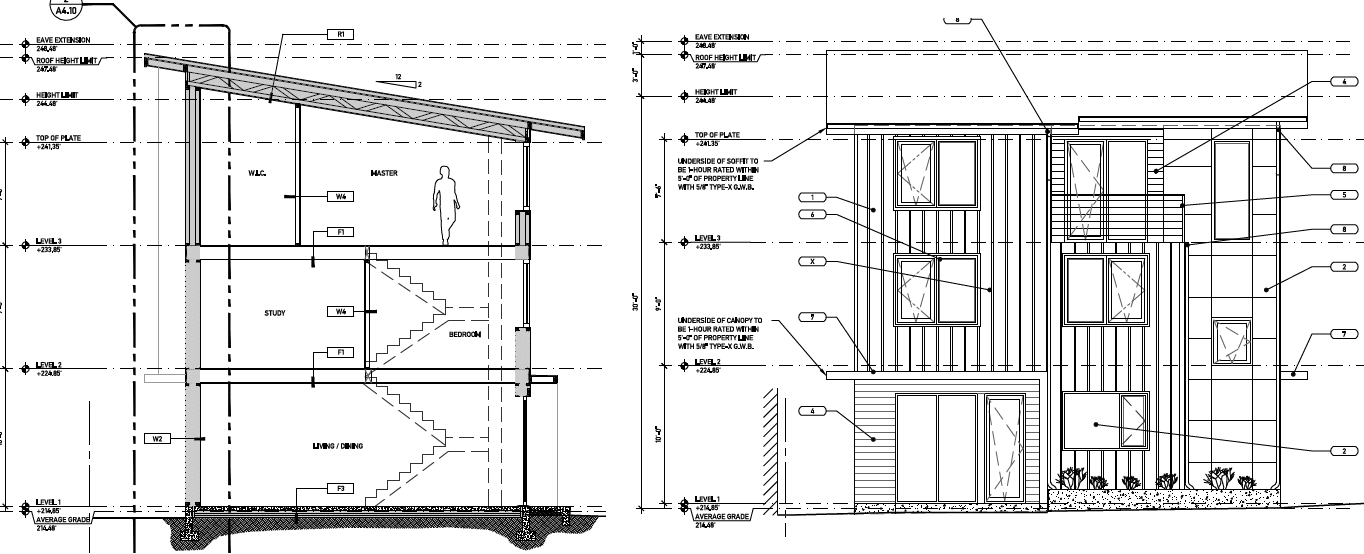
\includegraphics{case3.png}
\caption{Building plan of Case Study 3}
\end{figure}

\hypertarget{case-study-4}{%
\subsection{Case Study 4}\label{case-study-4}}

Case Study 4 represents a common residential house not solar-ready. It
was told that it took about 5 days to install the solar system in this
house. This house has several obstructions on the roof, which is complex
in shape, thus solar modules had to be installed in the multi-split
zones. In particular, south facing roof area was not enough to have all
the modules, thus the modules had to be installed on the other sides, on
the east facing and west facing roofs. Thirteen modules were installed
on west, twelve on south and ten on east. Even the solar modules
installed on the south facing root had to be split into three zones
(two, four and six modules separately). The roof pitch is 8/12 and
roofing material is composition, which led to roof penetration during
installation. The roof shape made hard to secure access pathways around
the solar modules. Conduit for the solar system is run outside wall.
Tie-offs were installed when the work for the rooftop solar had started.
The characteristics of the house is typical around the area. The
comparisons of the case studies are in the table below.

\begin{table}[t]

\caption{\label{tab:unnamed-chunk-5}Summary of case studies}
\centering
\begin{tabular}{l|l|l|l|l}
\hline
Description & Case 1 & Case 2 & Case 3 & Case 4\\
\hline
Feature & 5 star built green & 5 star built green & Emerald star & Common\\
\hline
\multicolumn{5}{l}{\textbf{Solar zone}}\\
\hline
\hspace{1em}One continuous zone & Yes & Yes & Yes & No\\
\hline
\hspace{1em}No obstruction & Yes & No & Yes & No\\
\hline
\hspace{1em}Roofing material & Composition & Metal & Metal & Composition\\
\hline
\hspace{1em}No penetration & No & Yes & Yes & No\\
\hline
\hspace{1em}Pitch & 4/12 & 8/12 & 2/12 & 8/12\\
\hline
\hspace{1em}Roof area (L x W) & 22' x 36' & 20' x 38' & 33' x 34' & Multi-split\\
\hline
\hspace{1em}Roof area (sqft) & 792 & 760 & 1122 & 1282\\
\hline
\hspace{1em}Solar area (sqft) & 505 & 487 & 523 & 631\\
\hline
\hspace{1em}Solar zone ratio & 0.64 & 0.64 & 0.47 & 0.49\\
\hline
\multicolumn{5}{l}{\textbf{Solar system}}\\
\hline
\hspace{1em}PV (ea) & 28 & 27 & 29 & 35\\
\hline
\hspace{1em}A module (W) & 230 & 270 & 280 & 300\\
\hline
\hspace{1em}Capacity (kW) & 6.44 & 7.29 & 8.1 & 10.5\\
\hline
\hspace{1em}System weights (lbs) & 1176 & 1134 & 1218 & 1502\\
\hline
\hspace{1em}lbs/ sqft (estimated) & 2.39 & 2.39 & 2.39 & 2.37\\
\hline
\hspace{1em}Inverter type & String & Micro & Mirco & Optimizer\\
\hline
\multicolumn{5}{l}{\textbf{Installation}}\\
\hline
\hspace{1em}Anchor point & Yes & Yes & Yes & No\\
\hline
\hspace{1em}Access to roof & Ladder & Ladder & Ladder & Ladder\\
\hline
\hspace{1em}Access pathways & No & Yes & Yes & No\\
\hline
\hspace{1em}Conduit & External & Internal & Internal & External\\
\hline
\hspace{1em}Time it takes (days) & Not sure & 3 & 2 & 5\\
\hline
\hspace{1em}Installed year & 2011 & 2014 & 2015 & 2018\\
\hline
\end{tabular}
\end{table}

\hypertarget{develop-a-ptd-design-checklist-and-bim-model-for-new-solar-ready-houses}{%
\section{Develop a PtD design checklist and BIM model for new
solar-ready
houses}\label{develop-a-ptd-design-checklist-and-bim-model-for-new-solar-ready-houses}}

Features encouraging safer conditions for installers to install a solar
system have been identified and verified through interviews, surveys and
case studies. These analyses result in a PtD design checklist for any
stakeholders including, but not limited to, architectural designers of
residential houses to refer to for occupational safety. The checklist
has six sections for solar zone area, solar zone material, solar zone
pitch, fall protection, access to roof, and electrical consideration for
the future solar system. Each section has concerns leading to the safer
working conditions. Modular solar system and standardized design
templates could even reduce the workload and coordination cost in
addition to the easier and faster installation. Solar zone pitch is
divided into two sections, flat and sloped roof in the checklist.
Conduit and inverter are the subareas of the section, electrical
considerations. It is expected that the checklist will lead to the
active involvement of designers to execute PtD during the design of the
solar-ready houses through pointing them out safety perspectives on
design. The checklist is attached in the appendix.

Furthermore, BIM model was developed as a benchmark of solar-ready
houses featuring the house design in favor of safer and more effective
ways to install the future solar system. As discussed in the previous
case studies, a simple roof shape encourages one continuous and spacious
solar zone, and safer working conditions. The figures below of the roof
shape of Case Study 2 in comparison of Case Study 4 illustrates well
about the significant difference of the simple roof shape.

\begin{figure}
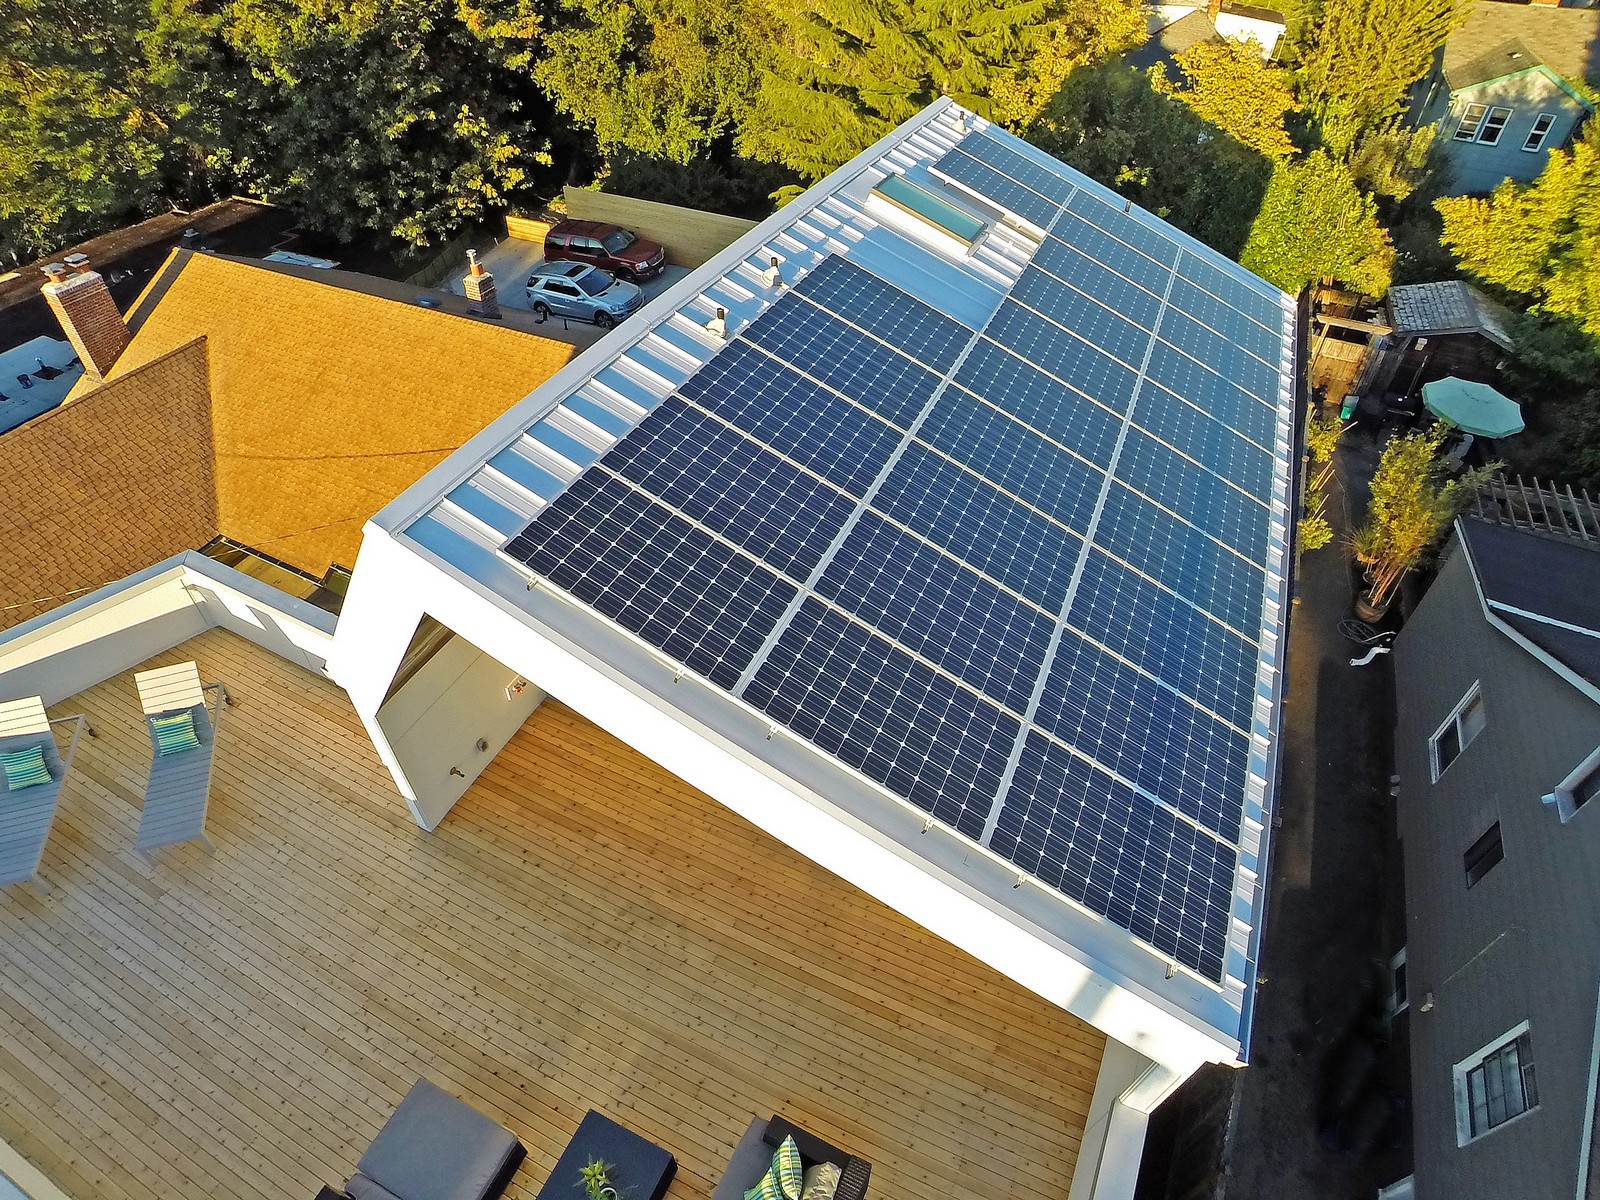
\includegraphics[width=3.2in]{../case/case2/dwelldevelopmentsolar2} 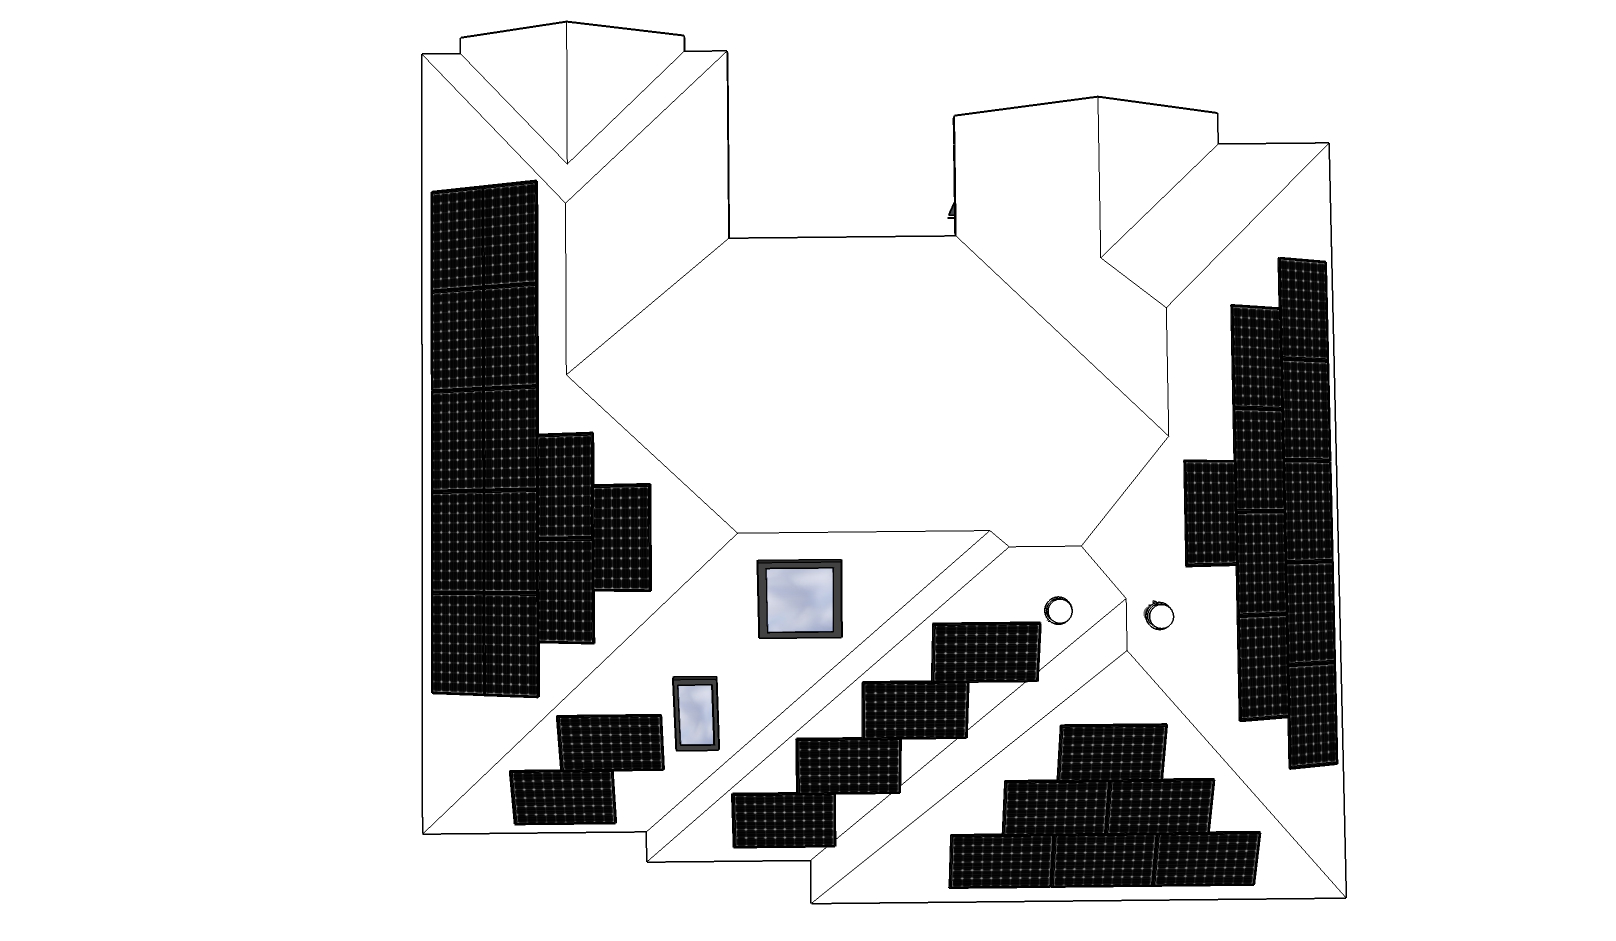
\includegraphics[width=4.04in]{../case/case4/ColorOH} \caption{Solar modules on roof of case studies 2 and 4}\label{fig:unnamed-chunk-6}
\end{figure}

Most of items in the checklist are applied to the BIM model. Access
pathways should be secured around solar zones and close to hip, valley,
eave and edge to make sure installers to move around during the work and
to prevent from falling. It is necessary to identify fall protection
measures such as guardrail around these area where it is easy to fall.
Metal (standing seam) or composition are suggested for roofing material
while avoiding tile and shake. It needs to check durability of the
roofing material, expected lifecycle for a solar system. Use of
composition should be avoided if a solar system goes more than 30 years
because common composition materials are known to be 30 years on average
in lifecycle and less durable than metal. Flat or lower-sloped roof are
recommended although flat roof may incur ballast mounting for a solar
system leading to structural engineering for dead and live load and
requiring a review of any intervention of solar system accessories with
membrane of the roof. Ballast mounting leads to carrying heavy weights
if necessary, on mechanical lifts in addition to ladders. Conduit is
suggested to run inside walls during new construction becuase it is
easier, safer, and more economical in addition to aesthetics in terms of
conduit pathways, inverter, and BOS locations. It is encouraged to have
all wiring systems (conduit and raceways for photovoltaic circuits)
close to ridge, hip or valley, if installed on walls. These safety
factors from the checklist are all applied to the benchmark model as
below (3ft access pathway around solar zone, tie-offs installed on roof
ridge, standing seam metal roof, lower-sloped roof, mechanical lift, and
conduit closed to ridge, hip or valley).

\begin{figure}
\centering
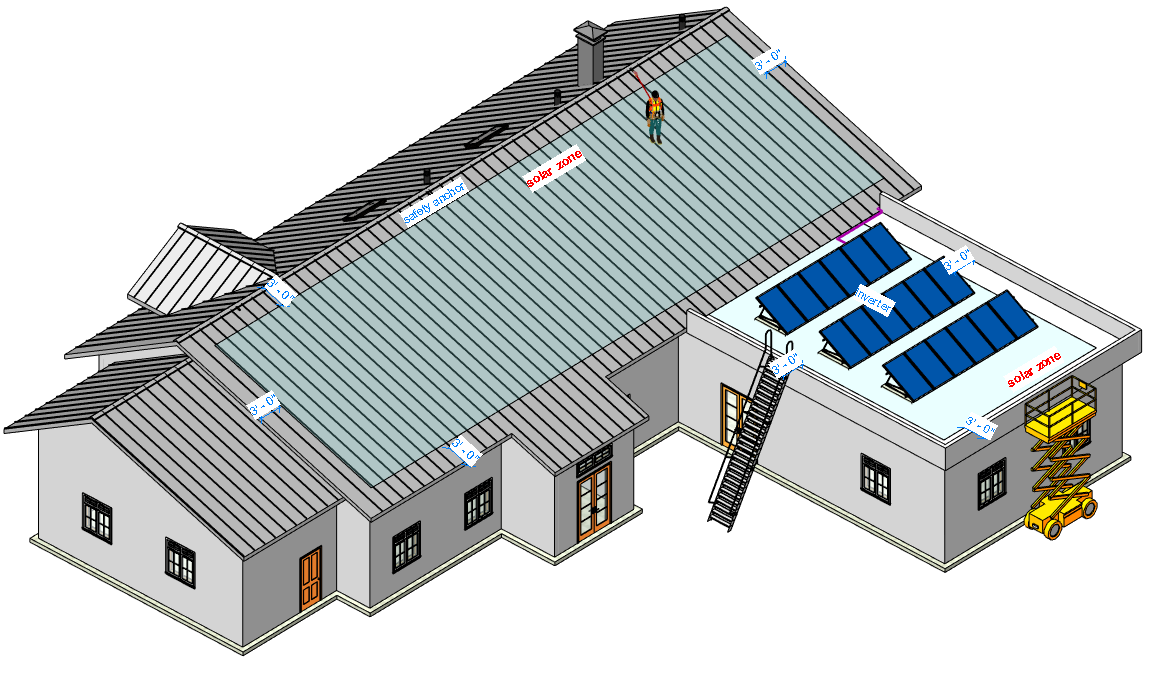
\includegraphics{3d_3.png}
\caption{3D model of the benchmark solar-ready house}
\end{figure}

\hypertarget{obtain-industry-feedback-on-the-checklist-and-model}{%
\section{Obtain industry feedback on the checklist and
model}\label{obtain-industry-feedback-on-the-checklist-and-model}}

On going..

\hypertarget{conclusion}{%
\section{Conclusion}\label{conclusion}}

Solar-ready houses have become the benchmark that every newly
constructed residential houses should follow in preparation of
installation of a solar system on the roof. Literature reviews on
several states' energy codes confirm this trend with IECC leading the
standard. California Energy Code (CEC) even exceeds the solar-ready
requirements of IECC. These solar-ready requirements, however, have
mainly focused on the energy production by securing solar zones for the
future installation of solar modules and lack considerations of
occupational safety of those who are going to install the system while
most of safety hazards in construction, are fall and trip. Furthermore,
it was found that promoting occupational safety, in fact, increases the
effectiveness of the solar-ready design in cost-effectiveness and
marketability in addition to the safety.

The interview results from the industry professionals, reported the
benefits of solar-ready design in terms of cost-effectiveness,
productivity, occupational safety, asset marketability, and green
adoption. The solar-ready design can largely contribute to lowering the
soft cost of solar systems by reducing time taken for system permitting,
pre-construction engineering, marketing, and installation (when
installers are at risk of being on the roof). It also helps increase the
installation productivity, leading to improving occupational safety by
promoting easy access, simple layout, fewer tripping hazards, and fewer
openings. Some interviewees pointed out that the solar-ready design can
enhance the value of the solar-ready houses due to the marketing of the
solar-ready features. There were some concerns raised about solar-ready
design. Specifically there was a concern that most federal tax credits
for residential solar are currently not applicable to solar-ready design
except for a rare case reported in Oregon energy trust EPS that provides
incentive to contractors. While there does not seem to be any more
incentive available for contractors in terms of applying solar-ready
design in new construction, the general trend in the industry is that
solar-ready design becomes required by the local residential building or
energy codes more and more over time.

PtD design features related to building components and solar system
features were verified and categorized through interviews and surveys to
help designers get involved in PtD for solar-ready houses. These
features include solar zone features, installation features and solar
system features. First, the solar zone features include solar zone area,
solar zone pitch, and solar zone material. Designers should consider
these features in terms of design constraints (e.g., rearranging
obstructions such as vents and chimneys) for the application of solar
zone as opposed to the typical rooftop design. Second, the installation
features are about how solar installers perform their installation in
terms of fall protection and access to roof. Lastly, the solar system
features are intended to address a time gap between solar-ready design
in the new construction and actual solar system installation in the
future. The identified solar features include electrical configuration
that determines the conduit routes and reserved spaces for electrical
components of the solar system depending on the inverter type.

The online survey verified the most desirable features for each criteria
of safety, applicability and cost-effectiveness. Furthermore, it was
found that there are conflicts among different objectives and features.
For example, optimal energy production requires 8/12 roof slope in
Northwest while the slope is not desirable for safety. Composition
roofing material is cheaper, but less durable, which may lead to
replacement of the roofing material in the middle of lifecycle of the
solar system on the roof. Flat roof in favor of safety may accompany
additional engineering cost and carrying heavy weights on the roof.
These trade-offs of the most desirable features were verified by the
four case studies consisting of the three solar-ready houses and one
common residential house.

The four case studies confirmed that the most desirable design features
for each building component. These design features promoting safer
conditions were applied to the PtD design checklist and BIM model for
designers to refer to for their active involvement of encouraging PtD on
design for safety. This study is unique in that it promotes safety in
solar-ready design while others mainly focus on securing solar zone to
make sure a certain level of energy production. Desirable safety
features suggested in this study different from the current solar-ready
requirements found in the general energy code such as IECC, are
including, but not limited to (1) access pathways around solar zone,
roof eave, and edges; (2) simple roof shape, modular solar system or
standardized roof design template preparing the roof for the future
solar system; (3) roofing materials of composition or metal standing
seam; (4) roof pitch of flat or lower-slope; (5) permanent installation
of fall protections; (6) strategic assessment of access to roof for
easier and effective ways; and (7) electrical considerations of conduit
pre-run and inverter options. These checklist and BIM model will help to
reduce safety hazards and mitigate risks by involving the designers in
the design development stage especially for green buildings pursuing
sustainability and energy efficiency.

\hypertarget{appendix---checklist}{%
\section{Appendix - checklist}\label{appendix---checklist}}

\hypertarget{solar-zone-area-1}{%
\subsection{Solar zone area}\label{solar-zone-area-1}}

\begin{itemize}
\tightlist
\item
  {[} {]} Consider a modular solar system (having roof ready for the
  future solar system) for easier and faster installation.
\item
  {[} {]} Take into account of standardized design templates\footnote{For
    example, integrative racking, process optimization, PV-ready
    electrical circuits, and conduit redesign.} in a packet to reduce
  coordination cost.
\item
  {[} {]} Design a simple roof shape with a designated solar zone
  (complex roof shape is only possible with compositions).
\item
  {[} {]} Have no obstructions around the solar zone to prevent tripping
  hazards.
\item
  {[} {]} Pre-install mounting accessories of a target solar system for
  future installation, considering penetration, flashing, and capped
  sleeve.
\item
  {[} {]} Designate access pathways\footnote{IFC 605.11.3.2.1
    Residential buildings with hip roof layouts. Panels/modules
    installed on residential buildings with hip roof layouts shall be
    located in a manner that provides a 3-foot-wide (914 mm) clear
    access pathway from the eave to the ridge on each roof slope where
    the panels/modules are located. The access pathway shall be located
    at a structurally strong location on the building capable of
    supporting the live load of fire fighters accessing the roof.
    (Exception: roof slopes ≤ 2:12). IFC 605.11.3.2.2 Residential
    buildings with a single ridge. Panels/modules installed on
    residential buildings with a single ridge shall be located in a
    manner that provides two, 3-foot-wide (914 mm) access pathways from
    the eave to the ridge on each roof slope where panels/modules are
    located (Exception: roof slopes ≤ 2:12). IFC 605.11.3.2.3
    Residential buildings with roof hips and valleys. Panels/modules
    installed on residential buildings with roof hips and valleys shall
    be located no closer than 18 inches to a hip or valley where
    panels/modules are to be placed on both sides of a hip or valley.
    Where panels are to be located on only one side of a hip or valley
    that is of equal length, the panels shall be permitted to be placed
    directly adjacent to the hip or valley. (Exception: roof slopes ≤
    2:12).} between the solar zone and the roof hip, valley, eave, or
  edge, to prevent fall hazards.
\end{itemize}

\hypertarget{solar-zone-material-1}{%
\subsection{Solar zone material}\label{solar-zone-material-1}}

\begin{itemize}
\tightlist
\item
  {[} {]} Avoid using materials such as tile and shake in the solar
  zone.
\item
  {[} {]} Check the material durability with respect to the expected
  lifespan of the solar system (if the system targets 30+ years, the use
  of composition should be avoided).
\item
  {[} {]} Select a roofing material in consideration of supporting bases
  such as flashing and penetration of the solar system.
\item
  {[} {]} Avoid using reflective materials to prevent heat stroke of
  workers in summer.
\item
  {[} {]} If metal roof is used, match the lip size of its standing
  seams to the clamp size of the solar system.
\end{itemize}

\hypertarget{solar-zone-pitch-1}{%
\subsection{Solar zone pitch}\label{solar-zone-pitch-1}}

\begin{itemize}
\tightlist
\item
  {[} {]} Apply flat to mild slope to the solar zone pitch.
\item
  {[} {]} Design a solar system layout with supporting bases in advance.
\end{itemize}

\hypertarget{flat-roof}{%
\subsubsection{Flat roof}\label{flat-roof}}

\begin{itemize}
\tightlist
\item
  {[} {]} Note that flat roof requires ballast mounting and
  TPO\footnote{Thermoplastic polyolefin, a single-ply roofing membrane
    covering the surface of the roof.} or other similar roof materials
  such as EPDM, PVC for the solar system.
\item
  {[} {]} Add additional load (at least 6 LB per square-foot) to
  structural engineering of the roof due to ballast mounting.
\item
  {[} {]} Review any interference of solar system accessories with roof
  membrane\footnote{Membrane on a flat roof: Minimum slope for water to
    run off is 1\% (1/8" per 1'). However, minimum slope for a flat roof
    by building code is 2\% (1/4" per 1'). A type of membrane roofing
    may be necessary.}.
\end{itemize}

\hypertarget{sloped-roof}{%
\subsubsection{Sloped roof}\label{sloped-roof}}

\begin{itemize}
\tightlist
\item
  {[} {]} Note that metal roof leads to slip hazards if it is
  considerably steep\footnote{Low-slop roof: OSHA defines a ``low-slope
    roof'' as a roof having a slope of less than or equal to 4 inches of
    vertical rise for every 12 inches horizontal length (4:12)
    (1926.500(b)---definitions).}.
\item
  {[} {]} Consider possibility of snow collection on the future system
  due to snow slide if the house is located in the snow climate.
\item
  {[} {]} Pre-assess access points and installation sequences for future
  solar system.
\end{itemize}

\hypertarget{fall-protection-1}{%
\subsection{Fall protection}\label{fall-protection-1}}

\begin{itemize}
\tightlist
\item
  {[} {]} Identify fall protection\footnote{OSHA 1926.501(b)(10):
    \ldots{} each employee engaged in roofing activities on low-slope
    roofs, with unprotected sides and edges 6 feet (1.8 m) or more above
    lower levels shall be protected from falling by guardrail systems,
    safety net systems, personal fall arrest systems, or a combination
    of warning line system and guardrail system, warning line system and
    safety net system, or warning line system and personal fall arrest
    system, or warning line system and safety monitoring system. Or, on
    roofs 50-feet (15.25 m) or less in width (see Appendix A to subpart
    M of this part), the use of a safety monitoring system alone
    {[}i.e.~without the warning line system{]} is permitted.} measures
  (such as guardrails\footnote{OSHA 1926.501(b)(11): \ldots{} Each
    employee on a steep roof with unprotected sides and edges 6 feet
    (1.8 m) or more above lower levels shall be protected from falling
    by guardrail systems with toeboards, safety net systems, or personal
    fall arrest systems.}) around roof hip, valley, eave, and edge.
\item
  {[} {]} Maintain setback pathways to hip, valley, eave and edge to
  prevent fall hazards.
\item
  {[} {]} Pre-install anchor points\footnote{Anchor point: OSHA standard
    regarding anchorages can be found in 29 CFR 1926.502(d)(15):
    Anchorages used for attachment of personal fall arrest equipment
    shall be independent of any anchorage being used to support or
    suspend platforms and capable of supporting at least 5,000 pounds
    (22.2 kN) per employee attached, or shall be designed, installed,
    and used as follows: 1926.502(d)(15)(i) as part of a complete
    personal fall arrest system which maintains a safety factor of at
    least two; and 1926.502(d)(15)(ii) under the supervision of a
    qualified person.}.
\item
  {[} {]} Develop a maintenance plan for the installed anchor points
  (there is a potential liability issue with pre-installed anchor
  point).
\item
  {[} {]} Consider additional options such as setback, snow
  guard\footnote{Rooftop devices that allow snow and ice to drop off in
    small amounts or allow snow and ice to melt completely before
    falling to the ground. The installation of snow guards prevents the
    sudden release of snow and ice from a roof, which is known as a roof
    avalanche. Snow guard could support installers and prevent them from
    falling.} and guardrail.
\end{itemize}

\hypertarget{access-to-roof-1}{%
\subsection{Access to roof}\label{access-to-roof-1}}

\begin{itemize}
\tightlist
\item
  {[} {]} Assess how to carry heavy materials (such as ballast mounting)
  to the roof.
\item
  {[} {]} Improve access through considering a lower height for the
  solar zone.
\item
  {[} {]} Improve access through considering a lower solar zone pitch.
\item
  {[} {]} Develop an access plan\footnote{IFC 605.11.3.1 Roof access
    point. Roof access points shall be located in areas that do not
    require the placement of ground ladders over openings such as
    windows or doors, and located at strong points of building
    construction in locations where the access point does not conflict
    with overhead obstructions such as tree limbs, wires, or signs.} for
  delivery of material and people in consideration of neighboring
  houses\footnote{Ladder: angle 75 degree, one-quarter the working
    length of the ladder (a 1:4 ratio) (29 CFR 1926.1053(b)(5)(i)). 3
    rungs (1 ft apart) above the roof, The side rails of the ladder
    generally must extend at least 3 feet above the upper landing
    surface that the worker is trying to access (29 CFR
    1926.1053(b)(1)).}.
\item
  {[} {]} Avoid having the solar zone under any overhead\footnote{IFC
    605.11.3.2.4 Residential buildings with smoke ventilation.
    Panels/modules installed on residential buildings shall be located
    no higher than 3 feet below the ridge in order to allow for fire
    department smoke ventilation operations.} powerline.
\end{itemize}

\hypertarget{electrical-considerations-for-the-future-solar-system}{%
\subsection{Electrical considerations for the future solar
system}\label{electrical-considerations-for-the-future-solar-system}}

\hypertarget{conduit}{%
\subsubsection{Conduit}\label{conduit}}

\begin{itemize}
\tightlist
\item
  {[} {]} Install wiring systems (conduit, raceways for photovoltaic
  circuits) close to ridge, hip or valley\footnote{IFC 605.11.1.2:
    Conduit, wiring systems, raceways for photovoltaic circuits shall be
    located as close as possible to the ridge or hip or valley, and from
    the hip or valley as directly as possible to outside wall to reduce
    trip hazard and maximize ventilation opportunity.}.
\item
  {[} {]} Pre-install conduit\footnote{Outside conduit: if protection
    sections are not more than 10 ft or 10 \% of the circuit length,
    then free air ampacities can be used. NEC 310.15(A)(2); if 4 - 6
    current carrying conductors are bundled in the same conduit, 80 \%
    adjustment is needed for conduit fill. NEC Table 310.15(B)(3)(a).
    Conduit spec: fill (NFPA 70 NEC, Article 310); type (NFPA 70 NEC,
    Article 690); size (NFPA 70 NEC, Article 300)} needed for a solar
  system.
\item
  {[} {]} Place conduit pathways, inverter, and balance of system
  (BOS)\footnote{The balance of system (BOS) encompasses all components
    of a photovoltaic system other than the photovoltaic panels.}
  locations in consideration of aesthetics.
\item
  {[} {]} Designate a space for electrical equipment on the same side as
  the solar system.
\end{itemize}

\hypertarget{inverter}{%
\subsubsection{Inverter}\label{inverter}}

\begin{itemize}
\tightlist
\item
  {[} {]} Consider a micro inverter or power optimizer for rapid
  shutdown\footnote{NEC rapid shutdown: The Section 690.12 update to the
    2017 National Electrical Code (NEC) calls for module-level rapid
    shutdown of solar systems instead of NEC 2014's array-level shutdown
    requirement. Starting Jan.~1, 2019 when NEC 2017 goes into effect in
    certain jurisdictions, all conductors within an array's 1-ft
    boundary have to be reduced to 80 V or less within 30 seconds of
    rapid shutdown initiation.} to avoid direct current (DC) electric
  shock\footnote{A fatal electrocution: a recent incident cited by OSHA
    about fatal electrocution leading to the company facing penalties at
    Kansas. OSHA Wichita Area Director, Ryan Hodge (2019) mentioned,
    ``This tragedy could have been prevented if the employer had
    complied with electrical standards that require maintaining a safe
    distance from unprotected energized power lines, training employees,
    and providing personal protective equipment.''}.
\item
  {[} {]} Consider a micro inverter or power optimizer for a small
  system about less than 35 modules for electrical safety in addition to
  cost-effectiveness.
\item
  {[} {]} Consider a string inverter to prevent tripping hazards and to
  reduce the time spent on roof for installation of a system about
  larger than 35 modules.
\end{itemize}

\hypertarget{appendix---bim}{%
\section{Appendix - BIM}\label{appendix---bim}}

\begin{figure}
\centering
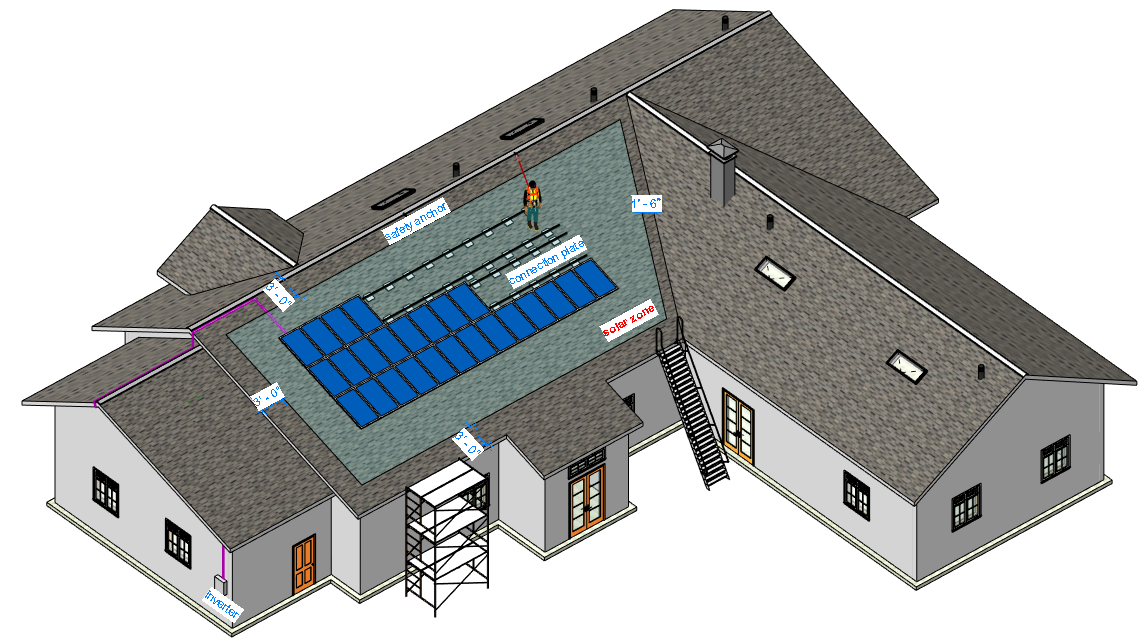
\includegraphics{3d_2.png}
\caption{3D model of the benchmark solar-ready house (composition roof)}
\end{figure}

\begin{figure}
\centering
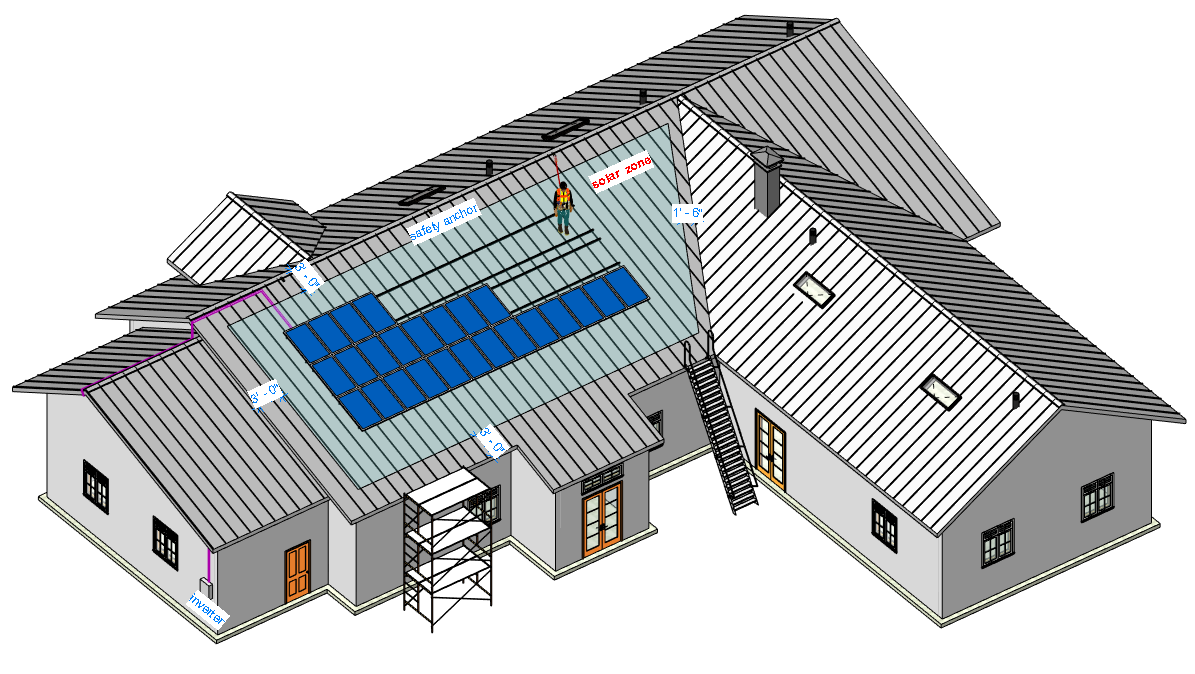
\includegraphics{3d_1.png}
\caption{3D model of the benchmark solar-ready house (metal roof)}
\end{figure}

\begin{figure}
\centering
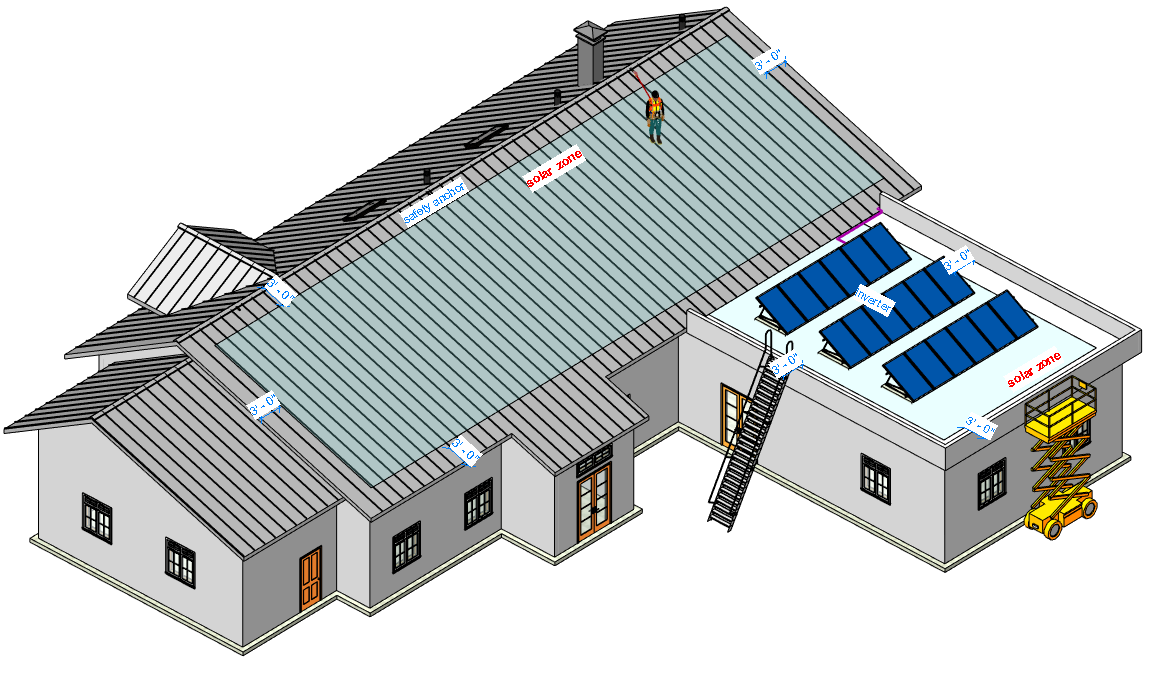
\includegraphics{3d_3.png}
\caption{3D model of the benchmark solar-ready house (flat and metal
roof from West South)}
\end{figure}

\begin{figure}
\centering
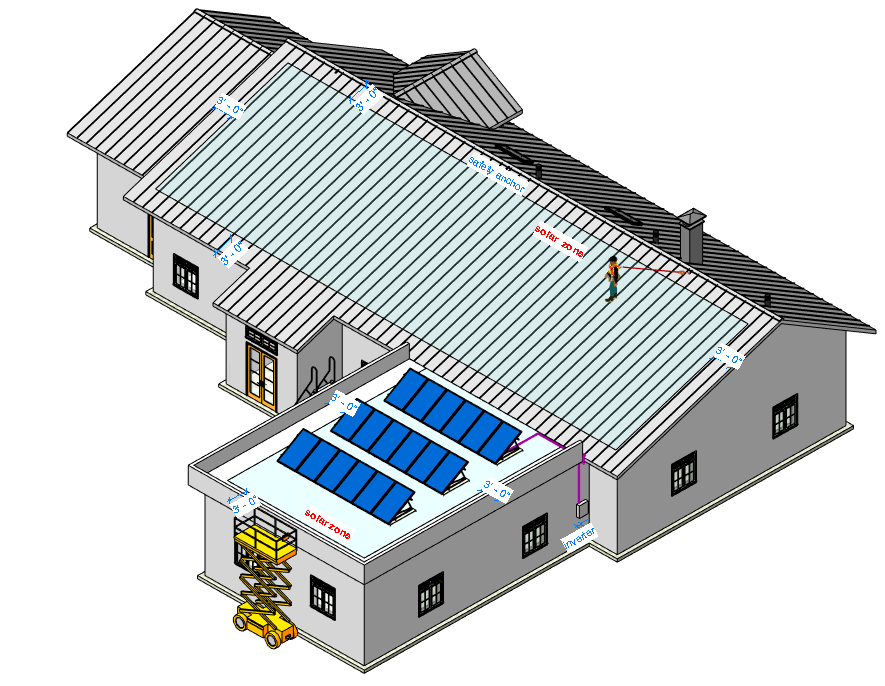
\includegraphics{3d_4.png}
\caption{3D model of the benchmark solar-ready house (flat and metal
roof from East South)}
\end{figure}

\hypertarget{references}{%
\section{References}\label{references}}

CPWR (2018). ``The Construction Chart Book.'' Sixth Edition. The Center
for Construction Research and Training (CPWR).
\url{https://www.cpwr.com/sites/default/files/publications/The_6th_Edition_Construction_eChart_Book.pdf}.

EPA (2011). ``Solar Photovoltaic: Specification, Checklist and Guide.''
Technical Report EPA-430-D- 110-01, US Environmental Protection Agency
(EPA).

GTM/SEIA (2017). ``GTM Research/SEIA U.S. Solar Market Insight -- 2016
Year in Review.'' GTM Research and Solar Energy Industries Association
(SEIA).

Harrington, R. (2015). ``The US is about to hit a big solar energy
milestone.'' Business Insider.
\url{http://www.businessinsider.com/solar-panels-one-million-houses-2015-10}

Lee, H.W., Gambatese, J., and Ho, C. (2017). ``Applying Prevention
through Design (PtD) to Solar Systems in Small Buildings.'' Final
Project Report. CPWR.
\url{https://www.cpwr.com/sites/default/files/publications/PtD-Solar-Solar-Systems-in-Small-Buildings.pdf}

Lisell, L., Tetreault, T., and Watson, A. (2009). ``Solar Ready
Buildings Planning Guide.'' Technical Report NREL/TP-7A2-46078, National
Renewable Energy Laboratory (NREL), US Department of Energy (DOE).

NY Daily News (2017). ``Worker installing solar panels dies after
falling from roof of two-story Queens house.'' Thursday, October 19,
2017.
\url{http://www.nydailynews.com/new-york/queens/workerdead-falling-roof-two-story-queens-house-article-1.3575395}

SEIA (2018). ``California Solar.'' Solar Energy Industries Association
(SEIA). \url{https://www.seia.org/state-solar-policy/california-solar}.

\hypertarget{refs}{}
\leavevmode\hypertarget{ref-cec2016BuildingEnergy2016}{}%
CEC. (2016). ``2016 Building Energy Efficiency Standards for Residential
and NonResidential Buildings.'' 289.

\leavevmode\hypertarget{ref-ecmSolarContractorCited2019}{}%
EC\&M. (2019). ``Solar Contractor Cited by OSHA After Fatal
Electrocution at Kansas Jobsite.'' \emph{Electrical Construction \&
Maintenance (EC\&M) Magazine},
\textless{}\url{https://www.ecmweb.com/safety/solar-contractor-cited-osha-after-fatal-electrocution-kansas-jobsite}\textgreater{}
(Jan. 19, 2019).

\leavevmode\hypertarget{ref-iecc2018InternationalEnergy2018}{}%
IECC. (2018). ``2018 International Energy Conservation Code.''
\textless{}\url{https://codes.iccsafe.org/content/iecc2018/appendix-ra-solar-ready-provisions-detached-one-and-two-family-dwellings-and-townhouses}\textgreater{}
(Nov. 20, 2018).

\leavevmode\hypertarget{ref-seattleResidentialCodeSDCI2017}{}%
Seattle. (2017). ``Residential Code - SDCI \textbar{} seattle.gov.''
\textless{}\url{http://www.seattle.gov/sdci/codes/codes-we-enforce-(a-z)/residential-code}\textgreater{}
(May 10, 2019).


\end{document}
